\documentclass[12pt, a4paper]{article}
\usepackage[top=2cm, bottom=2.5cm, left=2.5cm, right=2.5cm]{geometry}
\usepackage[utf8]{inputenc}
\usepackage{graphicx}
\usepackage{amsmath}
\usepackage{mathptmx}
\usepackage{physics}

\bibliographystyle{unsrt}

\title{New results concerning the wobbling properties of $^{183,187}Au$}
\author{Robert Poenaru}
\date{\today}


\begin{document}
\maketitle

\section{Introduction}

Two wobbling sequences have been identified in $^{183}$Au by Nandi et. al. \cite{nandi2020}. One sequence has two bands with states of negative parity (built on top of the odd $h_{9/2}$ proton) and two bands with states of positive parity (built on top of the odd $i_{13/2}$ proton). Both sequences are considered to have $n_w=0$ for the \textit{yrast} band and $n_w=1$ for the one-phonon wobbling band.


\begin{figure}[ht]
    \centering
    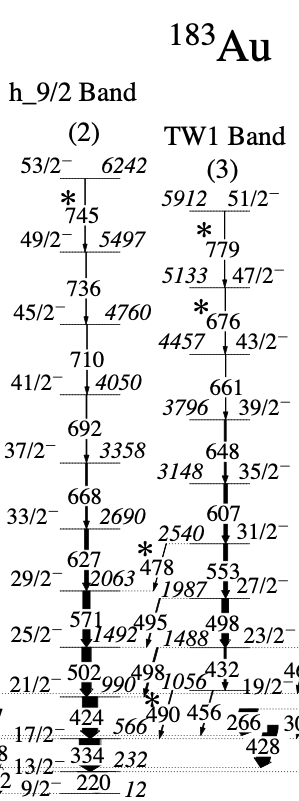
\includegraphics[scale=0.3]{figs/negative_Au183.png}\hspace{2cm}
    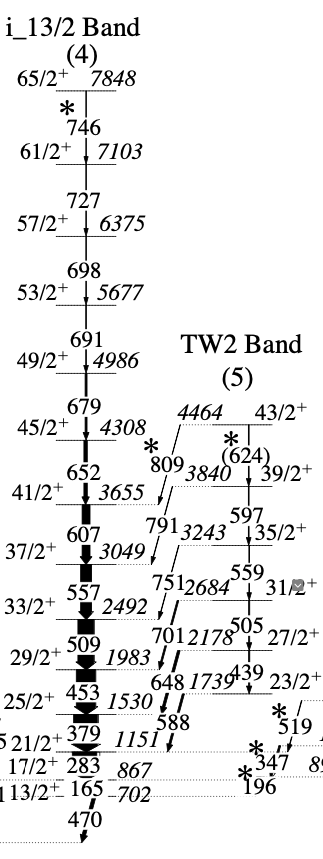
\includegraphics[scale=0.3]{figs/positive_Au183.png}\hspace{1.5cm}
    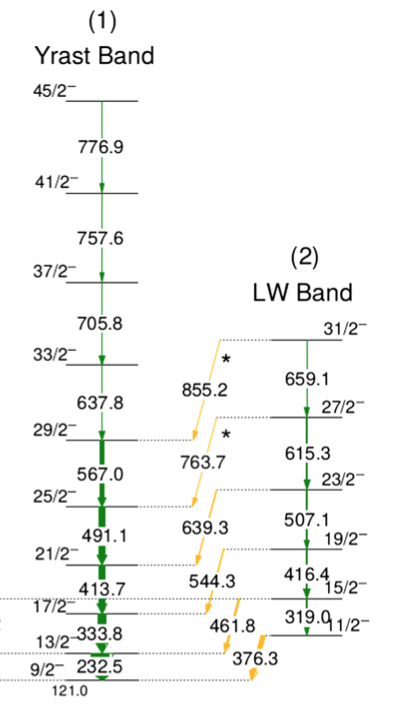
\includegraphics[scale=0.3]{figs/spectrum_Au187.png}
    \caption{\textbf{Left:} $^{183}$Au: negative parity states based on $j=9/2$.\textbf{Middle:} $^{183}$Au: positive parity states based on $j=13/2$. \textbf{Right:} The wobbling structure in $^{187}$Au.}
    \label{au_wobbling_bands}
\end{figure}

On the other hand, Sensharma et. al. \cite{sensharma2020} has confirmed wobbling motion in $^{187}$Au, with the identification of two such bands, show in figure \ref{au_wobbling_bands}.

\section{Numerical application}

By using the same formalism as the one applied for $^{163}$Lu in \cite{poenaru2021parity}. Namely, the both positive and negative wobbling sequences from $^{183}$Au were described with the same analytical expressions for the \textit{excitation energies}.

\newpage

\bibliography{references}

\end{document}